% -*- TeX:de -*-
\NeedsTeXFormat{LaTeX2e}
\documentclass[12pt,a4paper]{article}
\usepackage[german]{babel} % german text
\usepackage[DIV12]{typearea} % size of printable area
\usepackage[T1]{fontenc} % font encoding
%\usepackage[latin1]{inputenc} % most likely on Windows
\usepackage[utf8]{inputenc} % probably on Linux
\usepackage{multicol}

% PLOTTING
\usepackage{pgfplots} 
\usepackage{pgfplotstable}
\usepackage{url}
\usepackage{graphicx} % to include images
\usepackage{tikz}
\usepackage{subfigure} % for creating subfigures
\usepackage{amsmath} % a bunch of symbols
\usepackage{amssymb} % even more symbols
\usepackage{booktabs} % pretty tables
\usepackage{makecell} % multi row table heading

% a floating environment for circuits
\usepackage{float}
\usepackage{caption}

%\newfloat{circuit}{tbph}{circuits}
%\floatname{circuit}{Schaltplan}

% a floating environment for diagrams
%\newfloat{diagram}{tbph}{diagrams}
%\floatname{diagram}{Diagramm}

\selectlanguage{german} % use german

\begin{document}

%%%%%%% DECKBLATT %%%%%%%
\thispagestyle{empty}
			\begin{center}
			\Large{Fakultät für Physik}\\
			\end{center}
\begin{verbatim}


\end{verbatim}
							%Eintrag des Wintersemesters
			\begin{center}
			\textbf{\LARGE WS 2013/14}
			\end{center}
\begin{verbatim}


\end{verbatim}
			\begin{center}
			\textbf{\LARGE{Physikalisches Praktikum\\ für das Bachelorstudium}}
			\end{center}
\begin{verbatim}




\end{verbatim}

			\begin{center}
			\textbf{\LARGE{PROTOKOLL}}
			\end{center}
			
\begin{verbatim}

\end{verbatim}

			\begin{flushleft}
			\textbf{\Large{Experiment (Nr., Titel):}}\\
							%Experiment Nr. und Titel statt den Punkten eintragen
			\LARGE{PW10 Wechselstrom I}	
			\end{flushleft}

\begin{verbatim}

\end{verbatim}	
							%Eintragen des Abgabedatums, oder des Erstelldatums des Protokolls
			\begin{flushleft}
			\textbf{\Large{Datum:}} \Large{21.11.2013}
			\end{flushleft}
			
\begin{verbatim}
\end{verbatim}
							%Namen der Protokollschreiber
		\begin{flushleft}
			\textbf{\Large{Namen:}} \Large{Patrick Braun, Johannes Kurz}
			\end{flushleft}

\begin{verbatim}


\end{verbatim}
							%Kurstag und Gruppennummer, zb. Fr/5
			\begin{flushleft}
			\textbf{\Large{Kurstag/Gruppe:}} \Large{DO/2}
			\end{flushleft}

\begin{verbatim}

\end{verbatim}
							%Name des Betreuers, das Praktikum betreute.
			\begin{flushleft}
			\LARGE{\textbf{Betreuer:}}	\Large{Wilhelm Markowitsch}	
			\end{flushleft}

%%%%%%% DECKBLATT ENDE %%%%%%%
\pagebreak
\setlength{\columnsep}{20pt}
\begin{multicols}{2}

%%%%%%%%%%%%%%%%%%%%%%%%%%%%%%%%%%%%%%%%%%%%%%%%

%\begin{figure}[H]
%	\centering
%	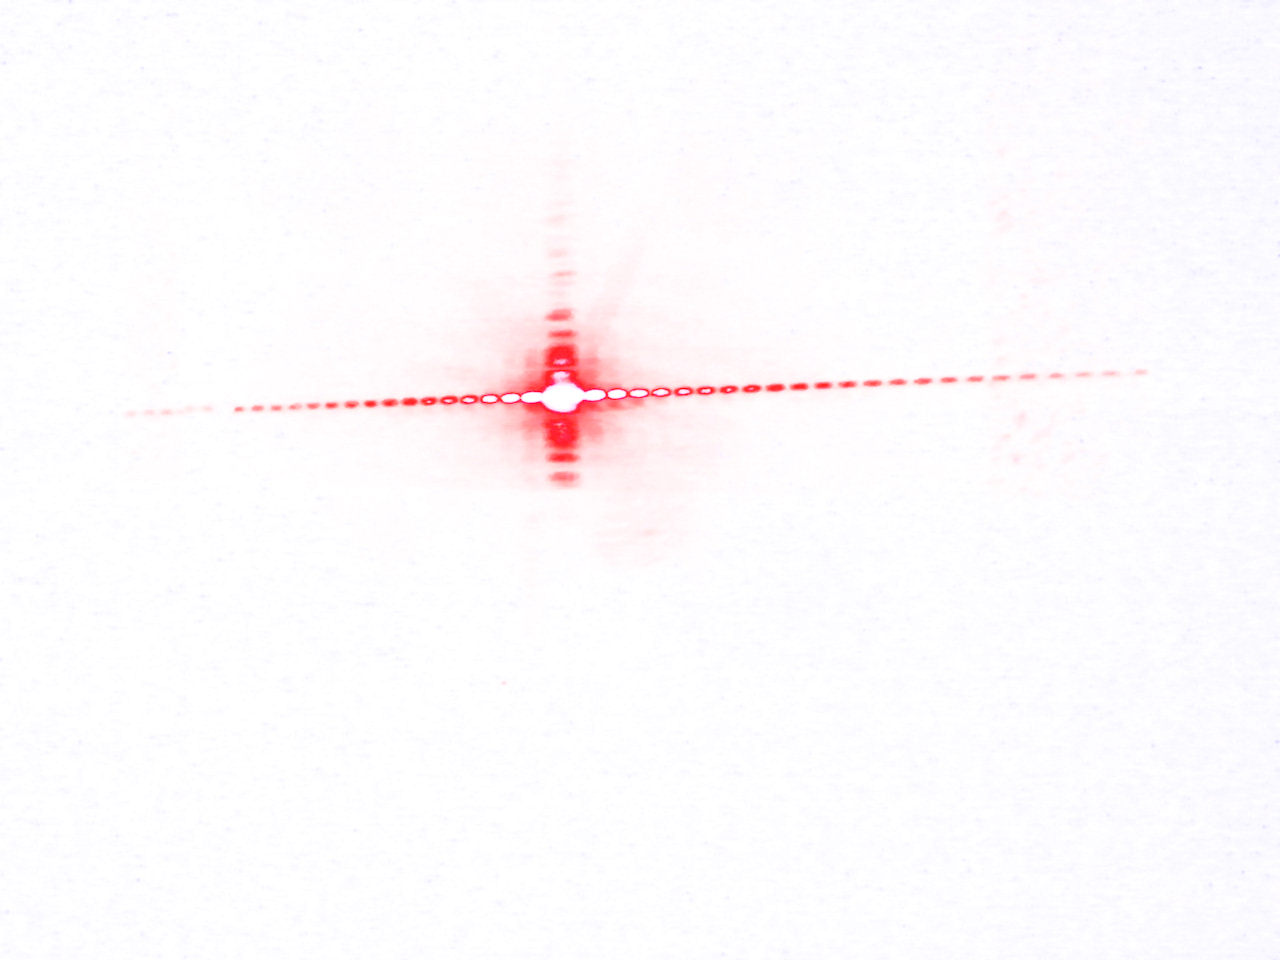
\includegraphics[scale=0.35]{./figure/beugung.png}
%	\caption{Beugungsmuster Einzelspalt (echtes Foto; schwarz durch weiß ersetzt)}
%	\label{fig:beugungsmuster}
%\end{figure}


%\begin{figure}[H]
%	\centering
%	\pgfplotstabletypeset[
%			columns={abstand, n},
%			col sep=&,
%			columns/abstand/.style={precision=2, zerofill, column name=\makecell{$Abstand$\\$(\pm 0.05)[mm]$} }, 
%			columns/n/.style={column name=\makecell{$n$\\$(Ordnung)$}, precision=0},
%			every head row/.style={before row=\hline,after row=\hline\hline},
%			every last row/.style={after row=\hline},
%			every first column/.style={column type/.add={|}{} },
%			every last column/.style={column type/.add={}{|} }
%			]{
%			abstand & n
%			12.9 & 1
%			24.45 & 2
%			37.40 & 3
%			49.35& 4
%			62.45 & 5
%			74.45 & 6
%			87.45 & 7
%			100.25 & 8
%			
%			}
%	\caption{Messwerte Einzelspalt}
%	\label{tab:werte_einzelspalt}
%\end{figure}
%


\section{Temperaturabhängigkeit des elektrischen Widerstandes}

Im ersten Teil von PW10 sollen die Widerstände 3er verschiedener Stoffe in Abhängigkeit der Temperatur bestimmt werden: Ein \textbf{Kaltleiter (PTC)}, ein  \textbf{Heißleiter (NTC)} und ein  \textbf{Elektrolyt}.
\\
Im Allgemeinen hängt der Widerstand (oder eben die Leitfähigkeit) eines Materials von der Zahl der freien Ladungsträger und deren Beweglichkeit ab. In PTC und NTC (also den Feststoffen) dienen als Ladungstäger die Elektronen im Leitungsband. Das ist derjenige Energie-Bereich, der über dem Valenzband liegt, dem höchsten, von Elektronen annähernd voll besetzten, Bereich.\\
\\
In Kaltleitern gehen diese Energieniveau-Bereiche ineinander über. Daher liegt der Grundzustand vieler Elektronen schon im Leitungsband. Steigt jedoch die Temperatur, schwingen die Atome stärker und behindern so die Bewegung der Elektronen. Der Widerstand steigt also mit steigender Temperatur.
\\
Dieser Effekt tritt auch bei Halbleitern (Heißleiter, NTC) auf, ist aber verschwindend gering, im Vergleich zur Steigerung der Leitfähigkeit mit zunehmender Temperatur: Die Elektronen in Halbleitern müssen eine gewisse Energielücke überwinden um vom Valenz- ins Leitungsband zu kommen. Steigt also die thermische Energie, steigt auch die Leitfähigkeit (exponentiell) an.
\\
In Fluiden können, im Gegensatz zu Feststoffen, Ionen oder sogar Moleküle Ladungsträger sein. Ihre Beweglichkeit hängt von der Viskosität ab. Diese nimmt exponentiell ab mit der Temperatur ab.
\\
Der Widerstand des Elektrolyts und des Halbleiters zeigen also eine ähnliche Temperaturabhängigkeit, wenn auch aus völlig verschiedenen Gründen.
\\
\begin{figure}[H]
	\centering
	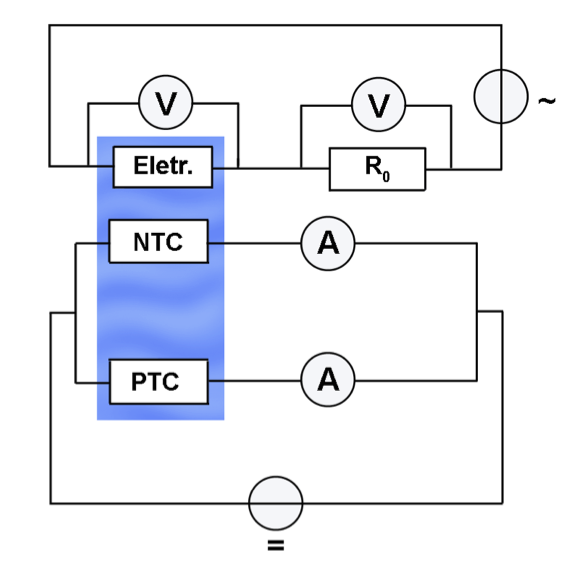
\includegraphics[scale=0.80]{./figure/schaltskizze_temp-widerst.png}
	\caption{Schaltskizze des Messaufbaus mit allen 3 Widerständen}
	\label{fig:schaltskizze_temp-widerst}
\end{figure}

Im Aufbau befinden sich alle 3 Widerstände in einem beheizbaren Wasserbad (destilliertes Wasser), mit einem Rührer, um die Temperatur des Wassers so gleichmäßig verteilt, wie möglich, zu halten.\\
NTC und PTC sind, in Parallelschaltung,  an eine 2V Gleichstrom-Spannungsquelle angeschlossen. An beiden Zweigen wird der Strom gemessen, durch den, mithilfe der konstanten Spannung, der Widerstand berechnet werden kann.\\
Mit dem Elektrolyt in Serie ist ein bekannter Widerstand $R_0$ geschaltet. An beiden wird die jeweils anliegende Spannung gemessen. Der Stromkreis wird mit 8V Wechselstrom betrieben.\\
Außerdem wird die Temperatur im Wasserbad gemessen.\\
Alle Messungen werden mit Cassy-Lab-Sensoren durchgeführt. Zuerst wird das Wasserbad auf etwa $80^\circ C$ erhitzt. Während dem Abkühlen werden die Messungen automatisch (2 Messungen/Minute) durchgeführt.\\
\\
\begin{itemize}
	\item \textbf{Elektrolyt}
	Die gemessenen Widerstände werden gegen die Temperatur aufgetragen. Durch einen Exponentialfit der Daten soll gezeigt werden, dass die exponentielle Beziehung tatsächlich gilt.\\
	Dabei soll in diesem Praktikumsbeispiel nicht näher auf die Viskosität eingegangen werden.
	
	\item \textbf{Halbleiter}
	Der Widerstand ist gegeben durch
	$$R(T)=R_{T_0}e^{-b\cdot (\frac{1}{T_0}- \frac{1}{T})}$$
	Durch Umformung erhalten wir die Geradengleichung:
	$$ln{\frac{R(T)}{R_{T_0}}}=b\cdot \frac{1}{T} + d$$
	wobei $R_{T_0}$ und $d$ miteinander in Beziehung stehen und hier nicht von Bedeutung sind.\\
	Die Lückenenergie $E_g$ des Halbleiters lässt sich aus dem Temperaturkoeffizienten $b$ berechnen:
	$$E_g = b \cdot 2k_B$$
	Von $E_g$ soll auf das verwendete Material geschlossen werden.
	
	\item \textbf{Kaltleiter}
	$$R(T) = R_{T_0} * [1+ \alpha (T - T_0)]$$
	$R(T)$ wird gegen $(T-T_0)$ aufgetragen ($T_0$ wird $20^\circ C$ gesetzt um mit der gegebenen Tabelle vergleichen zu können). \\
	Der y-Achsenabschnitt gibt $R_{T_0}$ und indem die Steigung der Gerade durch $R_{T_0}$ geteilt wird, erhalten wir den Temperaturkoeffizienten $\alpha_{20}$ für $20^\circ C$.\\
	Durch Vergleich soll der verwendete Leiter identifiziert werden.\\
	\\
		
\end{itemize}



\pagebreak

\subsection{Messwerte und Ergebnisse}
$U_{=} = (2.063 \pm 0.004)V$\\
\indent Gleichspannung (NTC \& PTC):\\
$T_0 = 20^\circ C$ gesetzt\\

%%%TO DO %%%%%%

%fehlerrechnung:



%Halbleiter:
% delta E_g = deltab * 2* boltzmanconstant



\end{multicols}
\noindent \textbf{Kaltleiter (PTC)}

\begin{figure}[H]
	\centering
	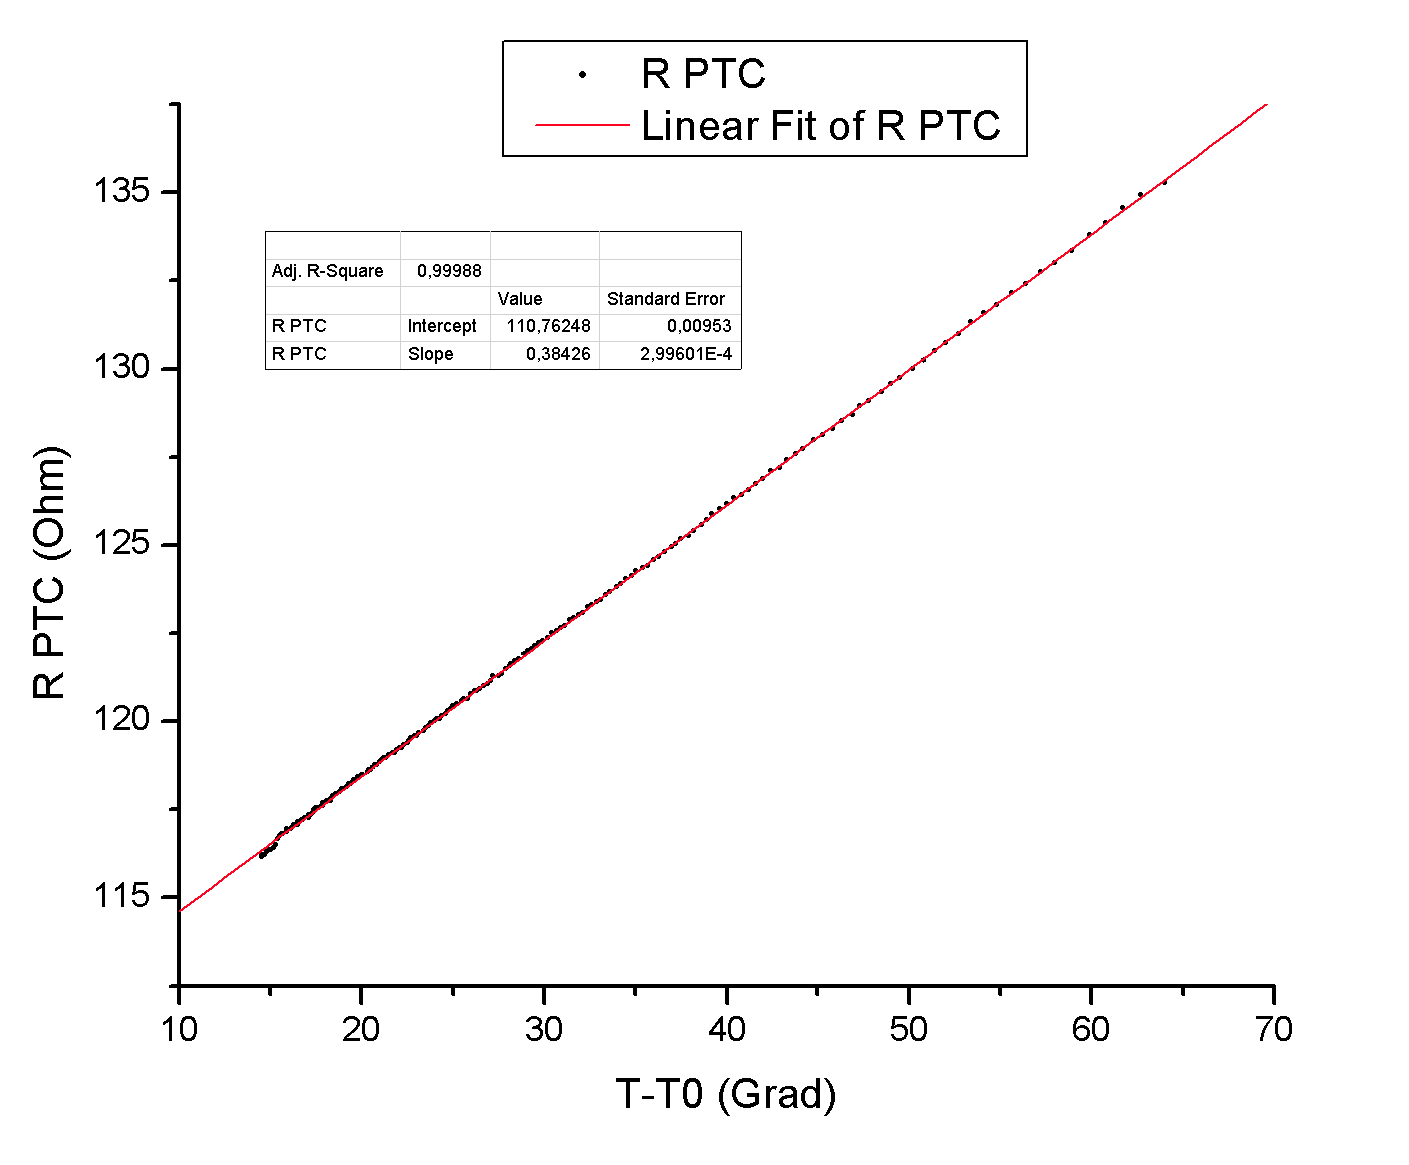
\includegraphics[scale=0.70]{./figure/RPTC_t_t0.png}
	\caption{Metal Widerstand mit linearem Fit}
	\label{fig:rptc}
\end{figure}

$$ \alpha_{20} = (3469.3 \pm  2.8    )K^{-1}$$
$$R_{T_0=20} = (110.76 \pm 0.01   )\Omega$$


Vermutung: Platin



\pagebreak



\noindent \textbf{Halbleiter (NTC)}


\begin{figure}[H]
	\centering
	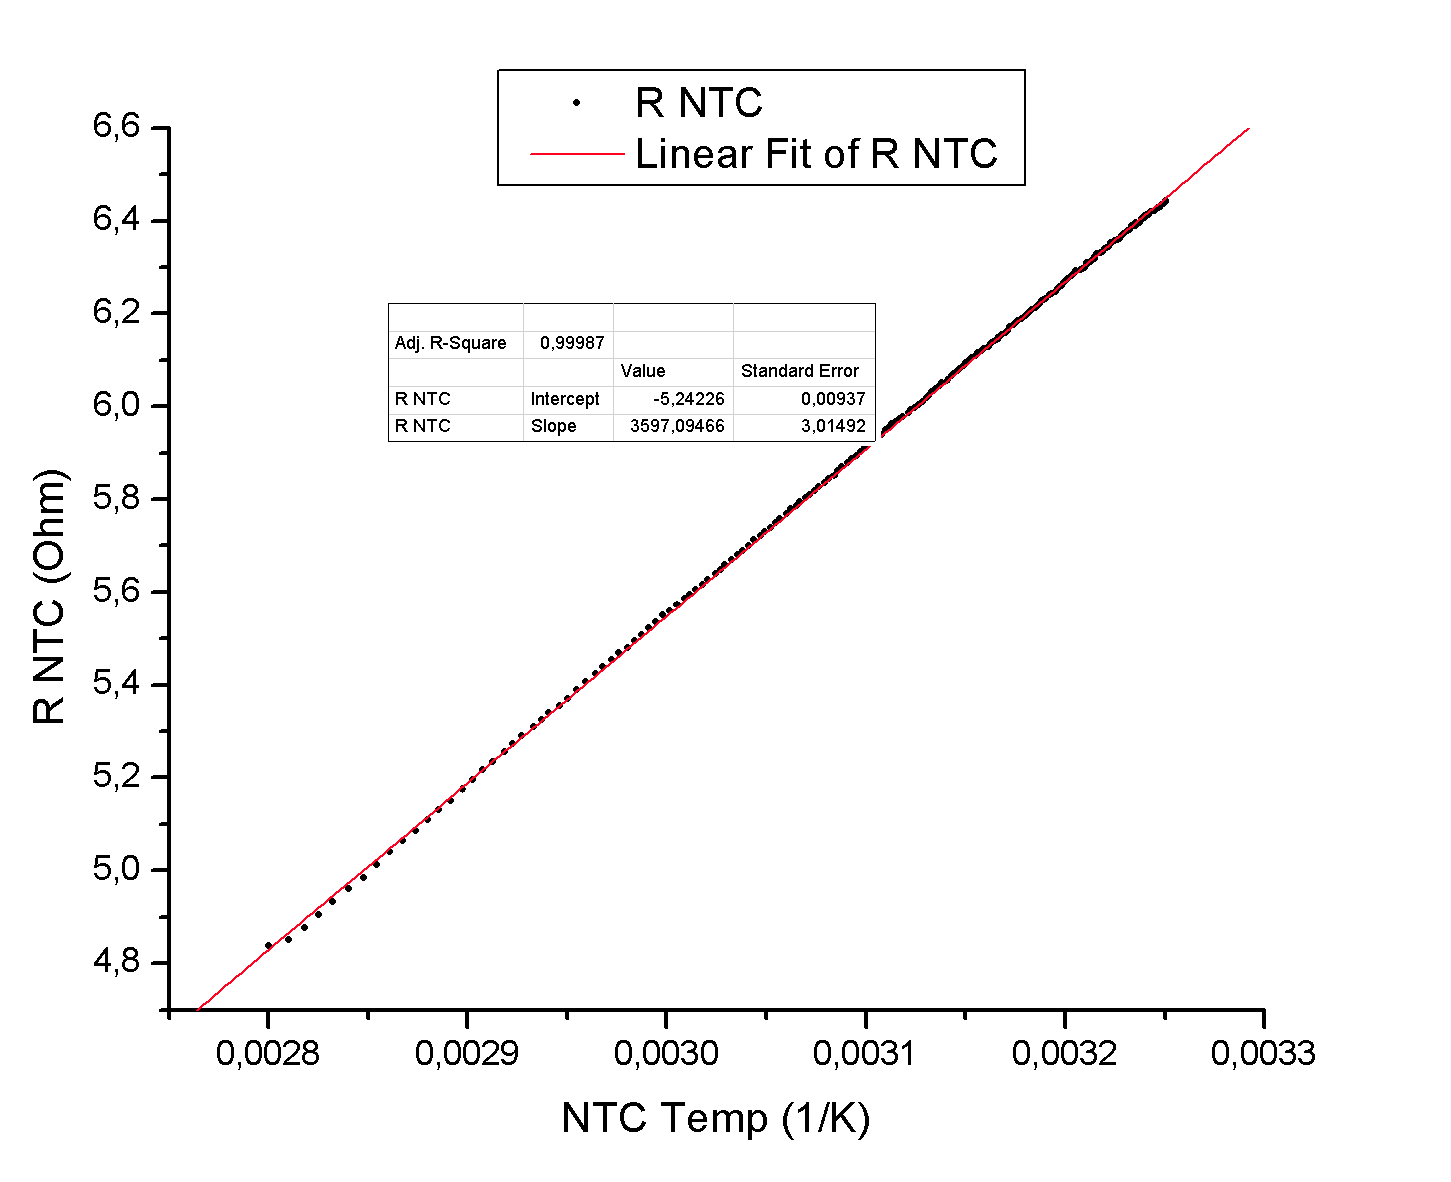
\includegraphics[scale=0.70]{./figure/RNTC_NTC_temp.png}
	\caption{Halbleiter Widerstand mit linearem Fit}
	\label{fig:rntc}
\end{figure}


 $$b = (3597.1 \pm  3.1   )K$$
$$E_g = (0.6198 \pm 0.0006   )eV$$

Vermutung: Germanium

\pagebreak


\noindent \textbf{Elektrolyt}

%% Kurve mit exp - fit

\begin{figure}[H]
	\centering
	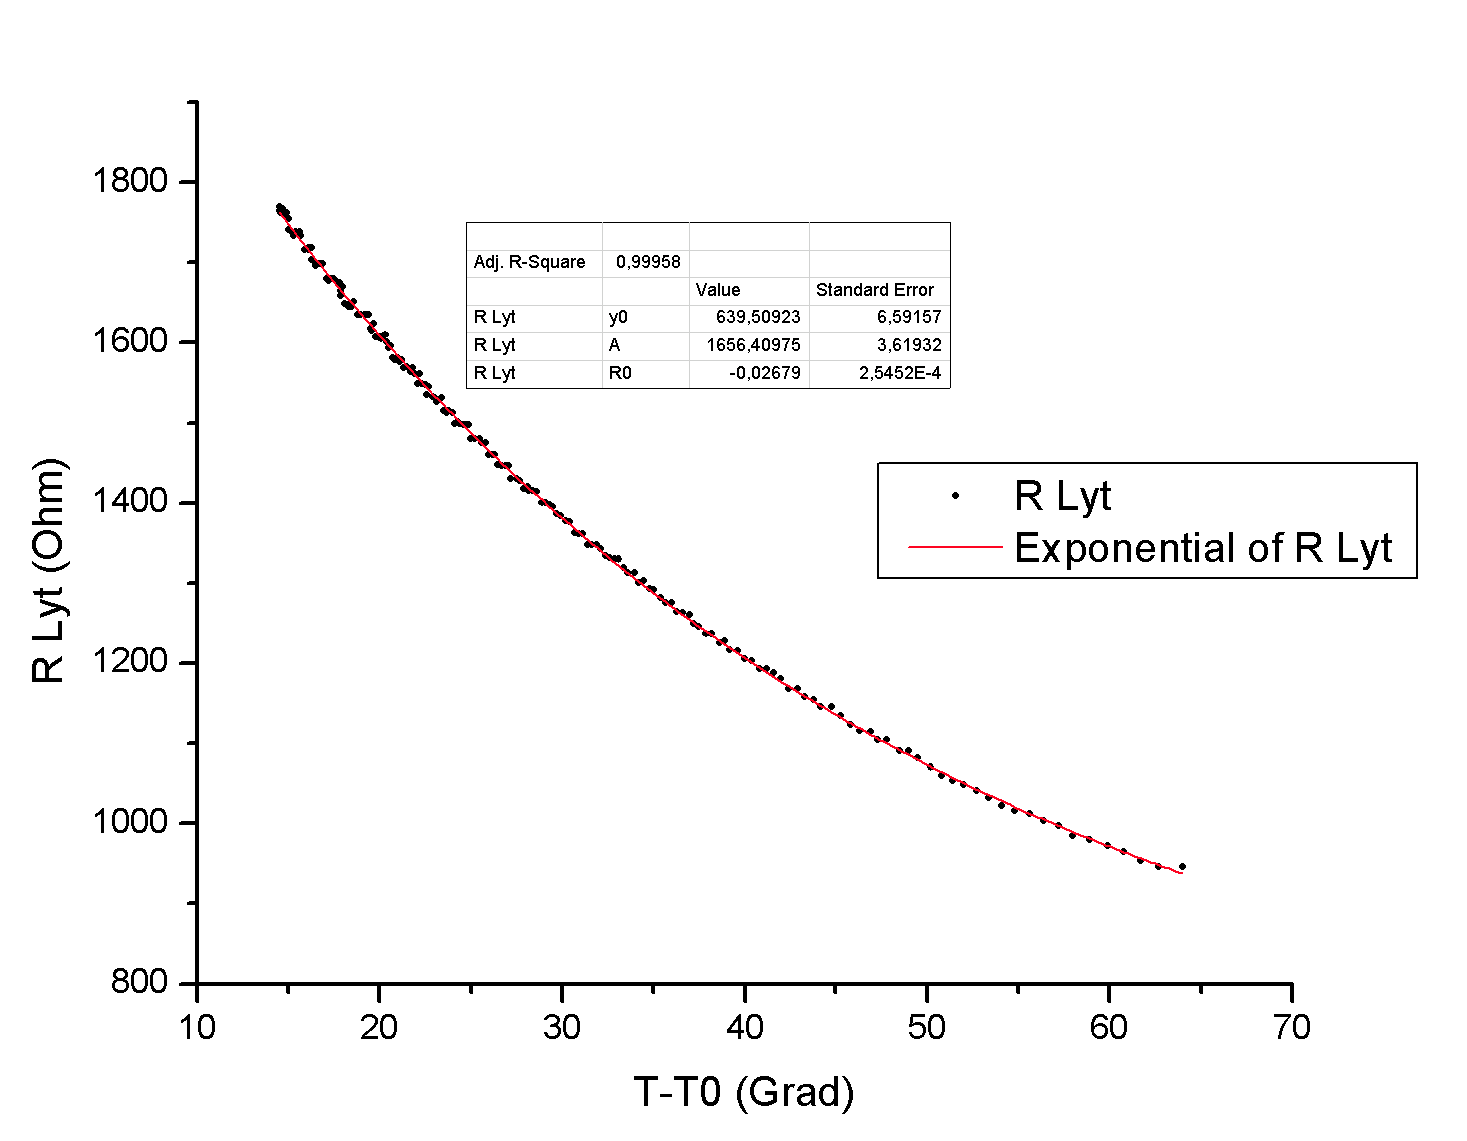
\includegraphics[scale=0.60]{./figure/Rlyt_t_t0.png}
	\caption{Widerstand Elektrolyt mit Exponentiellem Fit}
	\label{fig:rlyt}
\end{figure}



\begin{multicols}{2}
\subsection{Diskussion}

\textbf{(1) Kaltleiter:}
Der gemessene Temperaturkoeffizient $\alpha_{20}$ entspricht in der Tabelle der Praktikumsanleitung ([1], S.7) am ehesten demjenigen von Platin:\\
$\alpha_{Platin}= 3800K^{-1}$\\
Dies wurde auch, nach der Auswertung, vom Betreuer bestätigt.\\
Dennoch, der Literaturwert liegt deutlich außerhalb der Messunsicherheit des Ergebnisses. Da die einzelnen Messpunkte kaum von der angelegten Gerade streuen (wodurch sich letztendlich der kleine Unsicherheitsbereich ergibt, Abb. \ref{Metal Widerstand mit linearem Fit}), besteht die Vermutung, dass sich ein oder mehrere systematische Fehler im Versuchsaufbau befinden.\\
Ohne Wiederholung, Änderungen oder genauere Untersuchungen, lässt sich dazu zwar keine genaue Aussage treffen, mögliche Ursachen jedoch wären die Zusammensetzung des Leiters (verunreinigtes Platin) oder eine Abweichung der Leitertemperatur von der Wassertemperatur (Isolierung oder Kontakt zum Heizstab).\\
Nachdem auch die Theorie nur in Näherung gilt, ist möglicherweise auch hier eine Abweichung vom Literaturwert zu suchen.\\
\\
\textbf{(2) Heißleiter:}
Die gemessene Gap-Energy deutet auf Germanium hin:\\
Tabellenwerte ([1], S.5):\\
Ge: $0.75$ @ $0 ^\circ K$\\
$0.67$ @ $300 ^\circ K$\\
Auch das wurde vom Betreuer bestätigt.\\
Die Messung wurde von $80^\circ C$ bis etwa $35^\circ C$ gemacht, weswegen der gemessene Wert etwas niedriger liegt, als derjenige aus der Tabelle.\\
Auch die Einzelwerte dieser Messung liegen gut an der gefitteten Gerade und verdeutlichen somit die Theorie(Abb. \ref{Halbleiter Widerstand mit linearem Fit}).\\
\\
\textbf{(3) Elektrolyt}
In Abb. \ref{fig:rlyt} ist ein exponentieller Fit durch die gemessenen Widerstände, aufgetragen gegen die Temperatur. Es ist gut zu erkennen, dass auch für den Widerstand des Elektrolyts, abhängig von der Temperatur, ein exponentieller Verlauf gilt, wenn auch aus anderen Gründen, als im NTC.\\


%%%%%%%%%%%%%%%%%%%%%%%%%%%%%%%%%%%%%%%%%%%%%%%%
\section{Transformator}
In diesem Experiment soll das Verhalten eines Transformators untersucht werden. Dieser ist aufgebaut aus zwei Spulen (unterschiedlicher Windungszahlen), die um einen Eisenkern gewickelt sind. \\
In Abbildung \ref{fig:schaltung_trafo} ist der Versuchsaufbau mit dem Transformator, einem regelbarem Lastwiderstand und Messinstrumenten skizziert.



\begin{figure}[H]
	\centering
	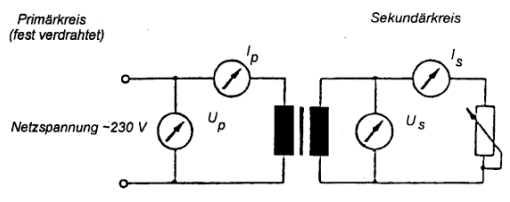
\includegraphics[scale=0.40]{./figure/schaltskizze_trafo.png}
	\caption{Versuchsanordnung zur Messung des Transformators (Quelle: [1](2.3))}
	\label{fig:schaltung_trafo}
\end{figure}


\noindent
Außerdem ist die \textbf{erzwungene} Netzspannung von 230V eingetragen. Die (in der Skizze links) anliegende Primärspannung $U_1$ bleibt also konstant. Wenn im sekundären Kreis (K2) mehr Leistung aufgenommen wird, und die Spannung im Primärkreis (K1) konstant gehalten wird, muss daher der Strom $I_1$ im K1 zunehmen.\\
\\
Die Übersetzung einer Spannung in eine andere, der wesentlichste Nutzen und Namensgeber von Transformatoren, erfolgt im Verhältnis der Windungszahlen der beiden Spulen:


$$\frac{U_1}{U_2} = -\frac{n_1}{n_2} = -u$$

\noindent
Aus Formel [1](9) ergibt sich, nach Einsetzen der Netzfrequenz für  $\omega$, folgende Berechnung der Induktivität $L_P$:

$$L_P = \frac{U_1}{I_1 * 2*\pi * 50Hz}$$

Dazu werden zuerst Primärspannung und -Strom gemessen, ohne einen angeschlossenen Lastwiderstand im Sekundärkreis.\\
Anschließend werden alle 4 Werte ($U_1, I_1, U_2, I_2$) für verschiedene Widerstände gemessen.





\subsection{Messwerte und Ergebnisse}

%$$u = -\frac{232.8V}{26.40V} = -8.81$$
$$u = (8.81 \pm 0.24)$$
\noindent
$|u| > 1 \Rightarrow$ die Spannung wird nach unten transformiert $\Rightarrow U_1 > U_2$ \\
\\
Induktivität $L_p$ der Primärspule:\\
%$$L_P = \frac{232.8V}{5.33mA *2*\pi * 50 Hz} = (139 \pm )H$$
$$L_P = (139.0 \pm 3.3)H$$

\end{multicols}
\begin{figure}[H]
	\centering
	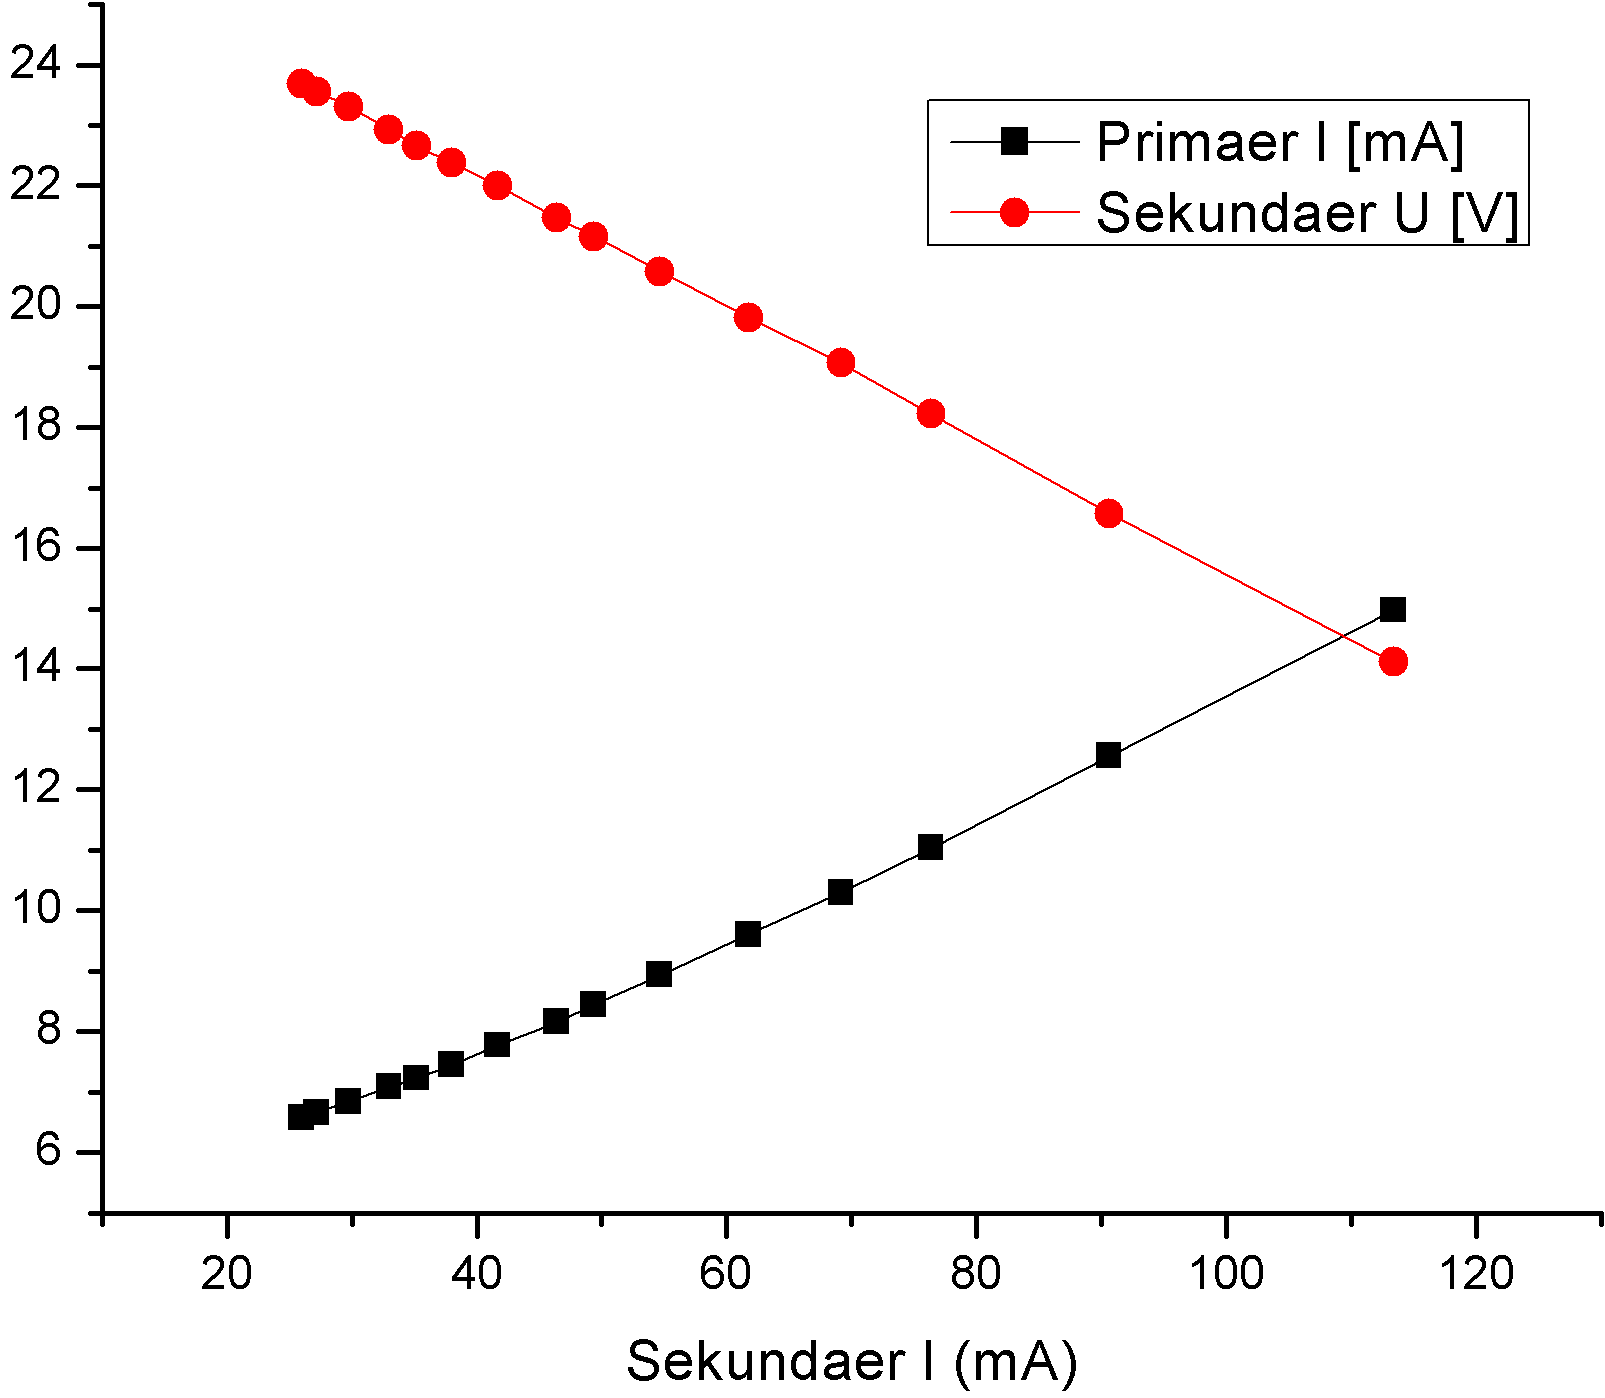
\includegraphics[scale=0.45]{./figure/transformator_sI_pI_su.png}
	\caption{Sekundärer Strom gegen primären Strom und sekundäre Spannung}
	\label{fig:trafo_si_pi_su}
\end{figure}
\begin{multicols}{2}

\end{multicols}
\begin{figure}[H]
	\centering
	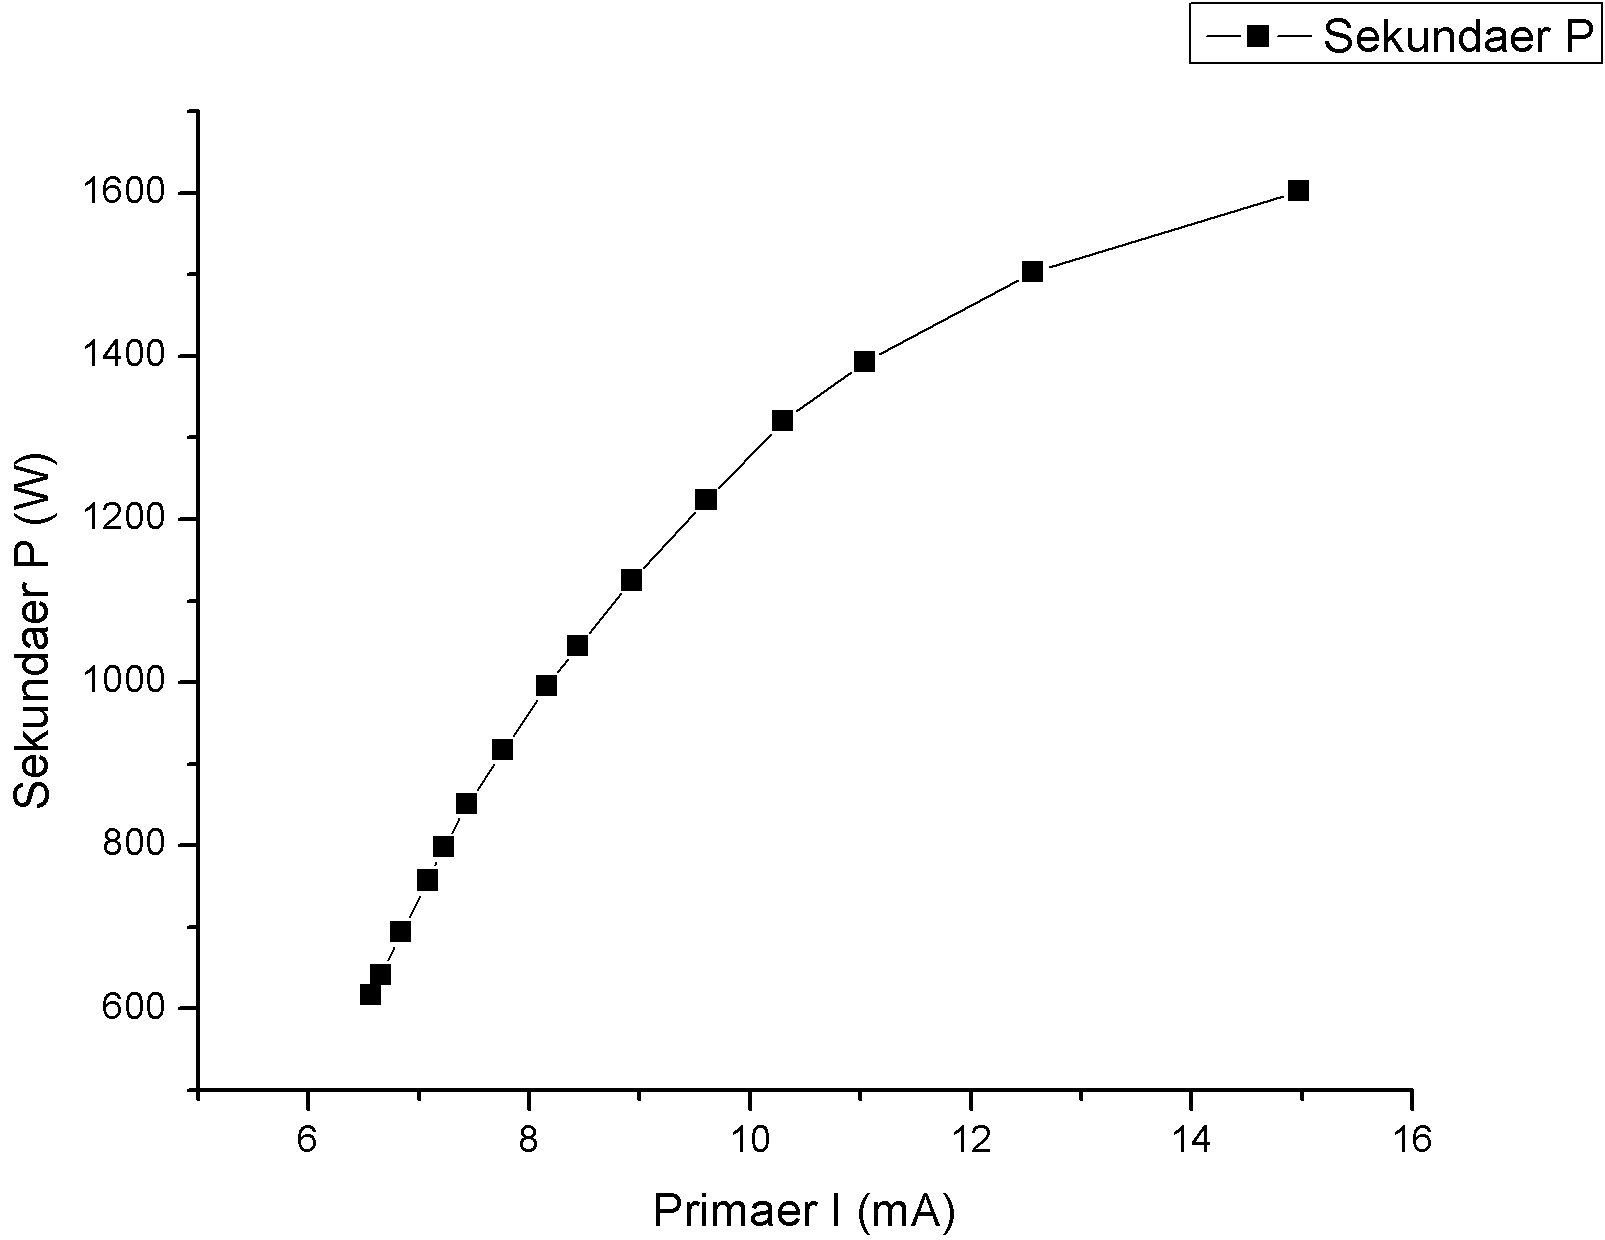
\includegraphics[scale=0.40]{./figure/transformator_pI_sP.png}
	\caption{Primärer Strom gegen sekundäre Leistung}
	\label{fig:trafo_pi_sp}
\end{figure}
\begin{multicols}{2}

\subsection{Diskussion}

In Abbildung \ref{fig:trafo_si_pi_su} ist zu sehen, dass bei höherer Belastung im $K2$, dank konstanter Spannungsversorgung im $K1$, der Primärstrom steigt.
Gleichzeitig fällt im K2 die Spannung ab.\\
Strom im K2 fließt nur dann, wenn der Transformator belastet wird (hier eben durch den Lastwiderstand). Dieser Strom $I_2$ induziert wieder ein B-Feld, das dem primären B-Feld entgegenwirkt. Diese Dämpfung des primären Feldes wird wiederum kompensiert, indem schlussendlich mehr Primärstrom $I_1$ fließen muss.\\
\\
Bei der Berechnung von $L_P$ ist der Widerstand rein (selbst)induktiv, da kein Abnehmer im K2 vorhanden ist, also kein weiteres B-Feld existiert (Ohmscher Widerstand der Leiter und Messgeräte vernachlässigt).\\
Nicht beeinflussbare Fehlerquellen bei der Messung sind beispielsweise Schwankungen der Netzspannung, ein nicht-lineares Verhalten des Regelwiderstandes sowie materialabhängige und bauliche Verluste im Transformator. Unvermeidbar sind zudem die Unsicherheiten der Messgeräte.\\
In Abbildung \ref{fig:trafo_pi_sp} ist die Leistung in $K2$ in Abhängigkeit vom Strom in $K1$ zu sehen. Bei hoher Leistungsaufnahme im $K2$, müsste der Strom in K1 gegen unendlich gehen, und damit die Leitungen überlasten (Überhitzung bzw. Abschalten durch eine Sicherung).
Optimalerweise sollte die Leistung nur bei kleinen Primärströmen entnommen werden, solange die Leistungskennlinie annähernd linear ist.\\
Die Phasenverschiebung ist im unbelasteten Fall 90$^\circ$ und im belasteten kleiner (Produkt ungleich 0).


%%%%%%%%%%%%%%%%%%%%%%%%%%%%%%%%%%%%%%%%%%%%%%%%%%


\section{Quellen}
$[1]$ Anleitung, \url{http://www.univie.ac.at/anfpra/neu1/pw/pw10/PW10.pdf}\\
$[2]$ 
\end{multicols}


\end{document}